\section{Design}
\label{sec:design}
\subsection{Application header-based Traffic Engineering}
\subsubsection{Q-in-Q}
\begin{comment}
\begin{figure}[htb!]
\includegraphics[width=1\columnwidth, trim={4cm 0cm 4cm 0cm}, angle=270,  scale=0.51] {figures/vlan_tag.pdf}
\caption{VLAN tag header insertion in Layer-2. 802.1Q was followed by 802.1ad in order to differentiate between customers on the same VLAN.}
\label{fig:vlan-tag}
\end{figure}
\end{comment}
%Figure \ref{fig:vlan-tag} 
%The IEEE 801.Q standard \cite{IEEE802.1Q:standard} describes the header frame format of the 802.1Q virtual LAN (VLAN) protocol, which was introduced in order to logically separate broadcast domains inside a Local Area Network (LAN). Following this, network service providers saw the need to similarly separate customers inside a VLAN and thus, a second 802.1Q tag was appended \cite{IEEE802.1ad:standard} to create Q-in-Q VLAN tunnels (802.1ad) that can easily be interpreted and altered by a network element with basic switching functionality. 
The IEEE 802.1ad standard \cite{IEEE802.1ad:standard} double-tagging was introduced to allow network service providers to separate traffic from different  VLANs as well as customers for better traffic management. Here, we use Q-in-Q tunneling to translate application-layer header information into link-layer headers at the edge before packets are forwarded to the core network. In particular, we focus on HTTP/2 application headers since they explicitly provide header fields that can be easily interpreted into Q-in-Q tags for better manageability.
\subsubsection{HTTP/2 Header}
\label{subsec:http2-header}
\begin{comment}
\begin{figure}[htb!]
%\centering
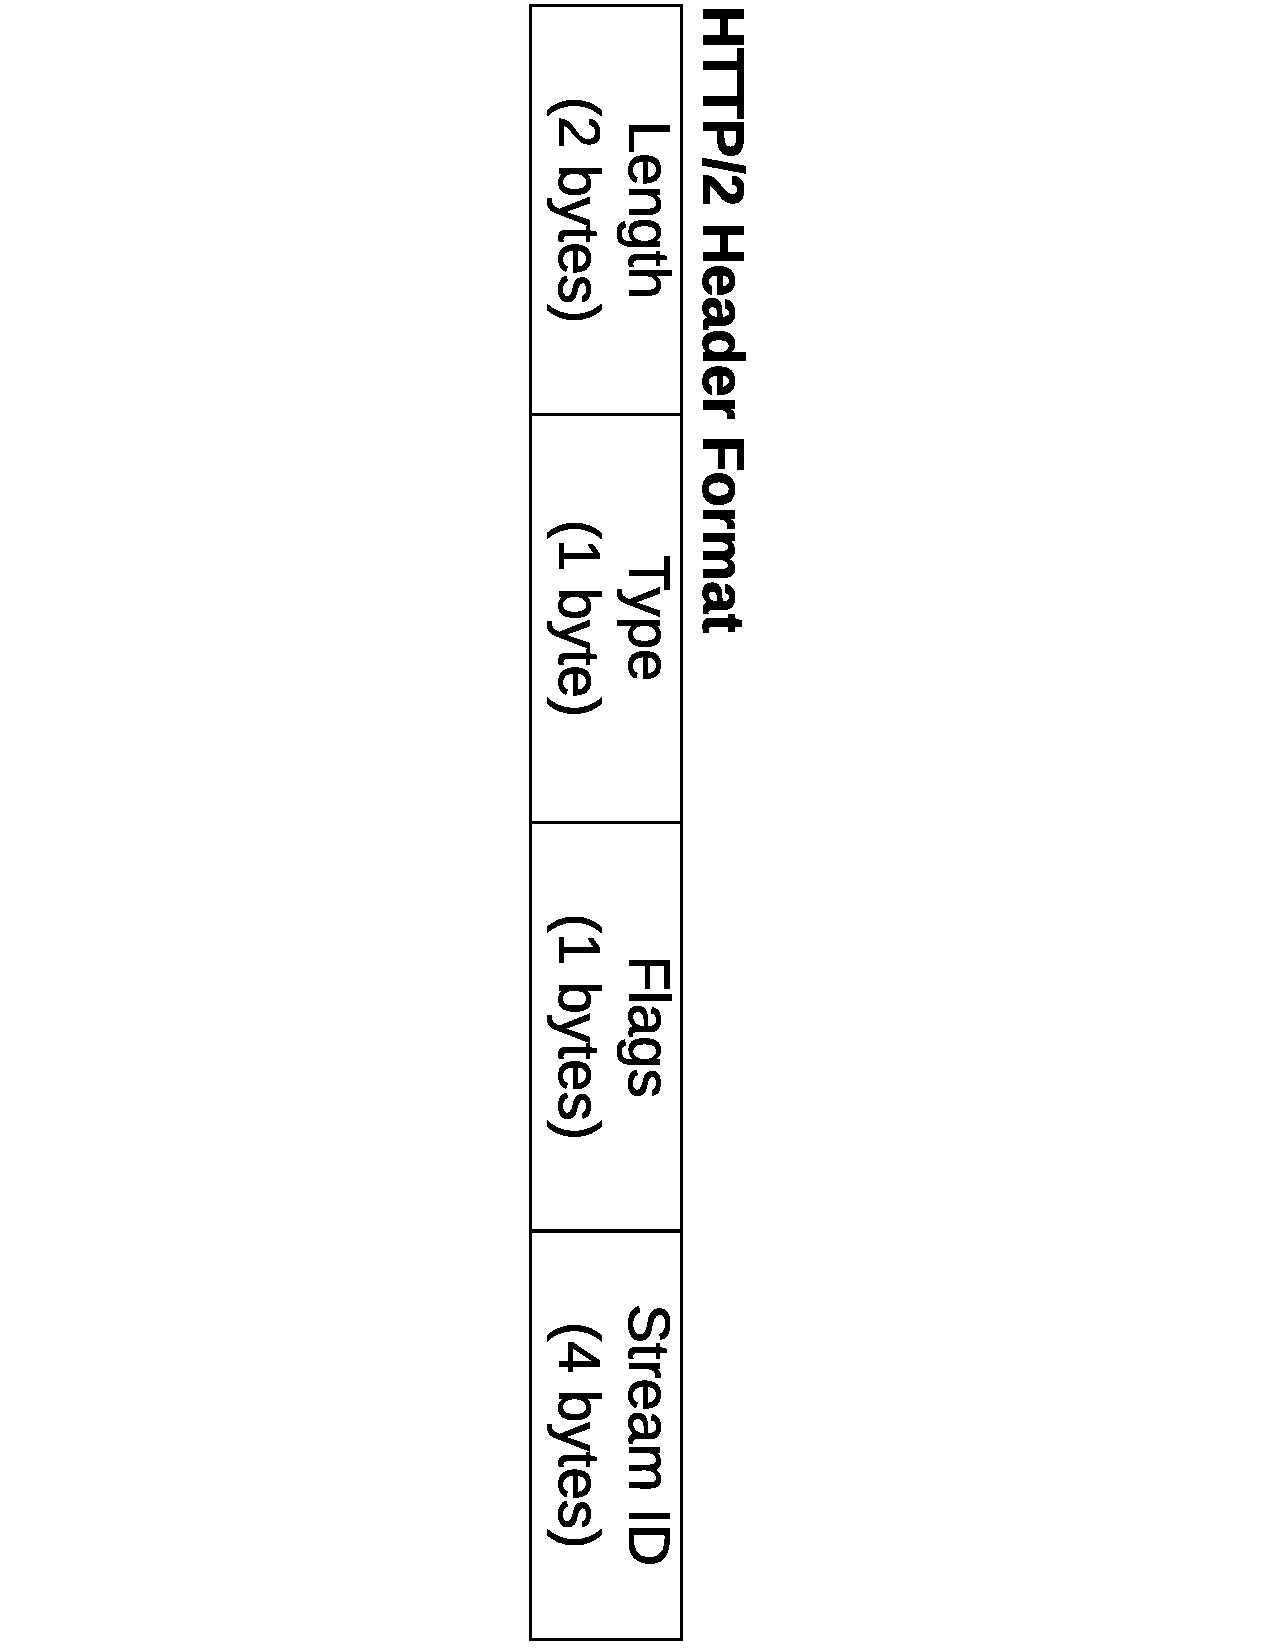
\includegraphics[width=1\columnwidth, trim={9cm 0cm 9cm 0cm}, angle=90, scale=0.13] {figures/HTTP2_header.pdf}
\caption{HTTP/2 Header Format: Common Eight-Byte Header}
\label{fig:http2-header}
\end{figure}
\end{comment}
As the number of objects embedded within a web page began to increase, the overhead due to variable length headers resulted in increased page load times for HTTP/1.1. Contrarily, HTTP/2 introduces a fixed length header and performs header compression in order to reduce perceived latency and increase goodput. It is interesting to note that HTTP/2 explicitly defines the \textit{Stream ID} field to multiplex several streams into a single TCP connection and thus, can be re-interpreted as a Q-in-Q tag by any link-layer device. %In general, the \textit{Stream ID} is used to differentiate between active concurrent downloads of embedded objects for a given web page.
In this work, we redefine the outer customer tag (C-TAG) as a \textit{Stream ID} tag using a flexible, protocol-independent packet processing language, P4 that can be programmed to interpret HTTP/2 headers. For the ABR video streaming application, \textit{Stream ID} is used to differentiate between two distinct bitrate qualities that are simultaneously downloaded by the client as described in our previous work \cite{acm-mmhttp2}. 
\subsection{System Architecture}
\begin{figure}
\vspace{-24pt}
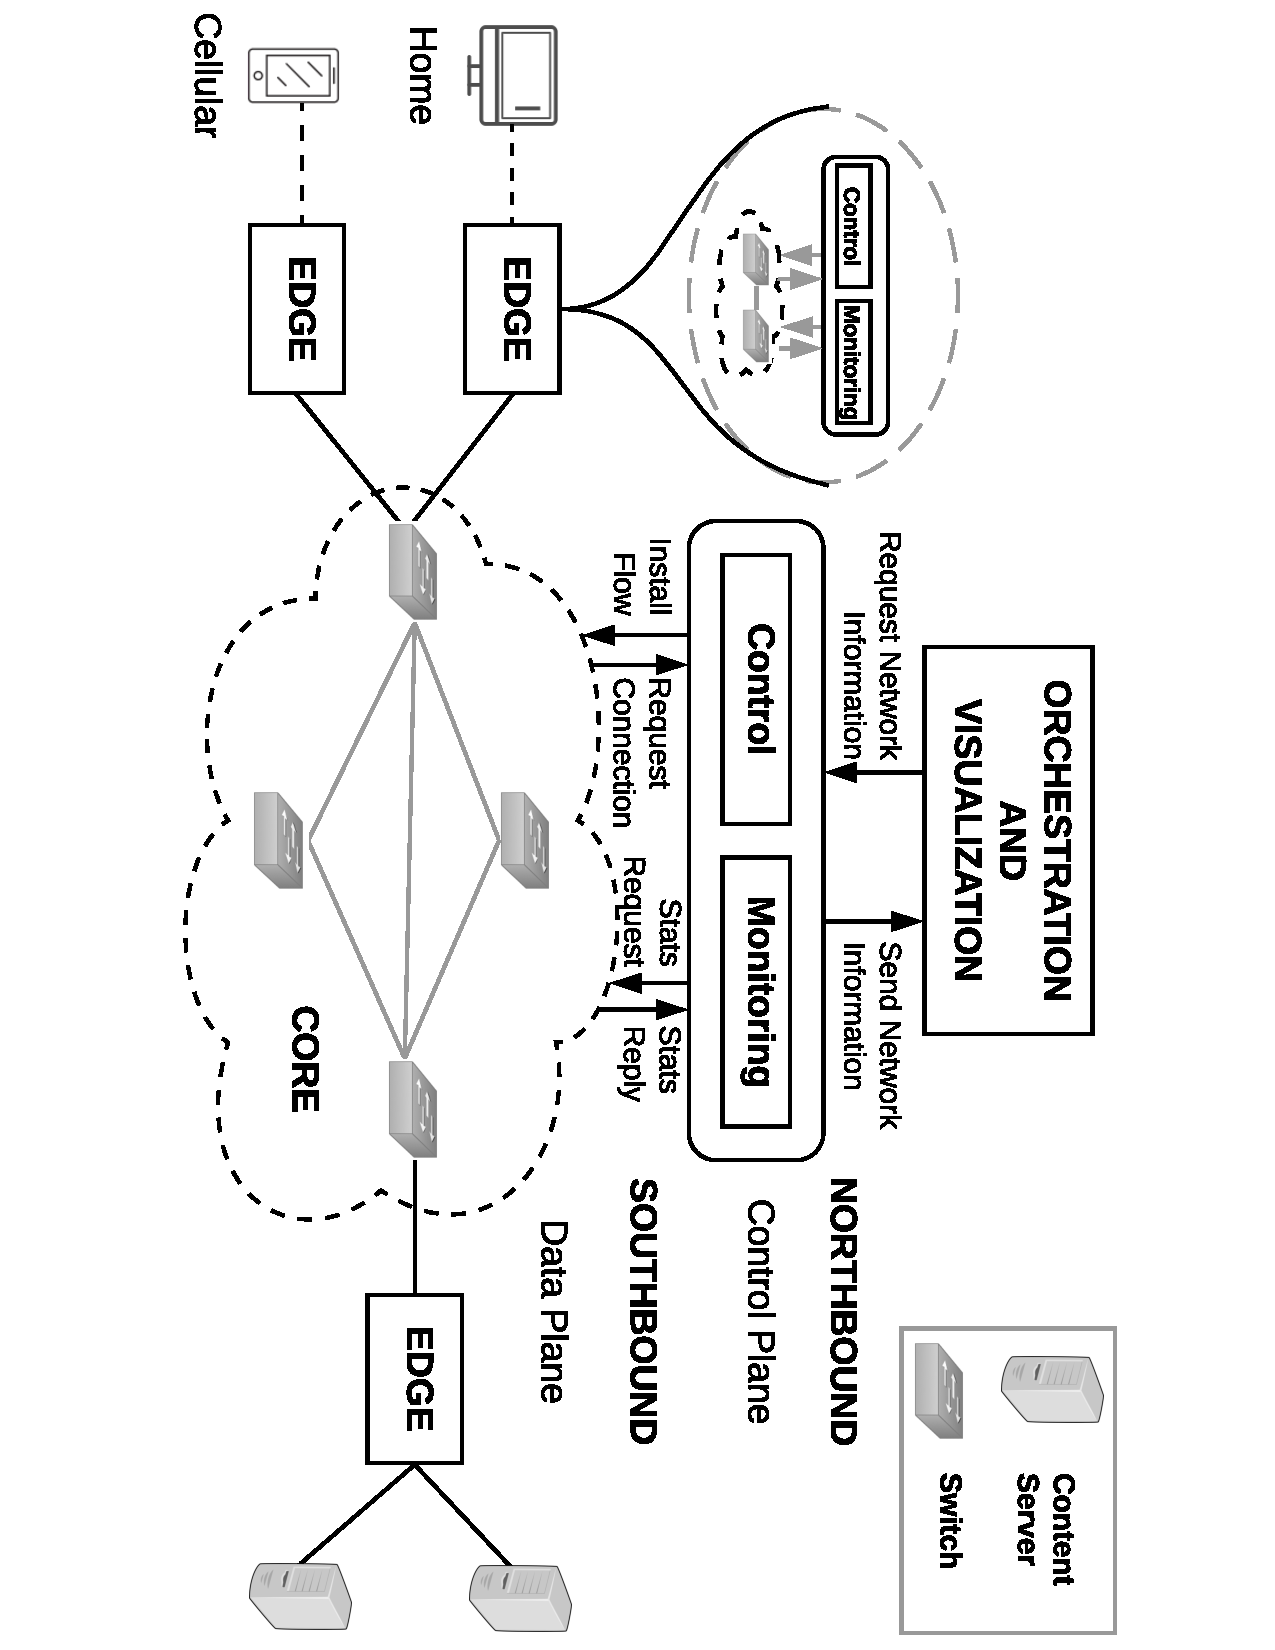
\includegraphics[ width=1\columnwidth, trim={2cm, 20cm, 0cm, 0cm}, angle=90, scale=0.7] {figures/NetworkArchitectureP4v2.pdf}
\caption{Architecture for QoE to QoS translation at the edge, which is envisioned as SD-WANs}
\label{fig:p4-of}
\vspace{-18pt}
\end{figure}
The main focus of our architecture is to translate application-layer header information into link-layer headers. We additionally includes a centralized component that allows network providers to orchestrate and visualize their network from a single interface.
Figure \ref{fig:p4-of} presents the architecture of our demonstration and consists of the following components:
\subsubsection{The Core}
For our architecture we assume a capability similar to that of a large-scale research testbed, ESNET\footnote{\url{https://www.es.net/network-r-and-d/experimental-network-testbeds/100g-sdn-testbed/}}, where the core or backbone network includes a programmable data-plane that performs fine-grained traffic engineering based on L2-L5 header information and is centrally controlled by an independent controller (denoted as \textit{Monitoring} and \textit{Control} in Fig. \ref{fig:p4-of}). However, we note that similar functionality can be incrementally deployed in production networks based on MPLS Traffic Engineering (MPLS-TE)\footnote{\url{https://www.cisco.com/c/en/us/products/collateral/ios-nx-os-software/multiprotocol-label-switching-traffic-engineering/}} techniques as well.
\subsubsection{The Edge}
Innovation at the edge such as SD-WANs \cite{Yap:2017} is driven by the tremendous growth in downstream application traffic and the advent of cloud computing. Here, the edge network also includes a programmable data-plane of several flexible switches that are centrally controlled by an independent controller. However, these switches can perform fine-grained traffic engineering using L5 header information as well. In order to peer with the core, the edge controller must translate information in L5 headers to L2-L4 headers before sending packets out into the core.
\subsubsection{Orchestration and Visualization}
Our system also includes a centralized component that aggregates monitoring information from the various controllers in order to provide a visual representation of network performance. 

The diagram also shows clients such as a wireless home network and cellular network that connect to an edge and receive requested content from a server located elsewhere on the edge network. The two edge networks are connected by the core. In the following section, we describe the setup for our demo including the platform and tools we use to run QoS translation experiments.


